% Created by tikzDevice version 0.12.3.1 on 2021-06-10 10:34:34
% !TEX encoding = UTF-8 Unicode
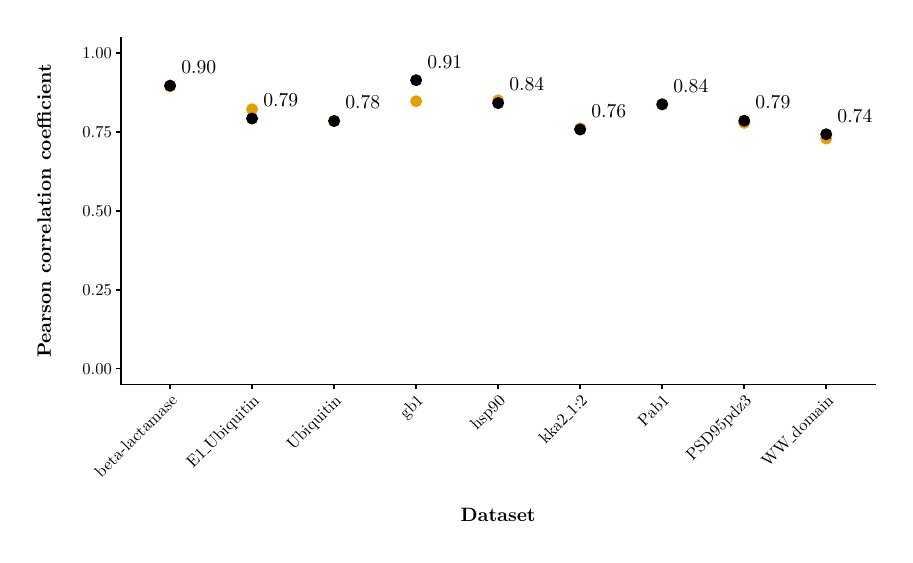
\begin{tikzpicture}[x=1pt,y=1pt]
\definecolor{fillColor}{RGB}{255,255,255}
\path[use as bounding box,fill=fillColor,fill opacity=0.00] (0,0) rectangle (309.84,183.39);
\begin{scope}
\path[clip] ( 33.67, 54.47) rectangle (306.34,179.89);
\definecolor{drawColor}{RGB}{230,159,0}
\definecolor{fillColor}{RGB}{230,159,0}

\path[draw=drawColor,line width= 0.4pt,line join=round,line cap=round,fill=fillColor] ( 81.09,153.92) circle (  1.96);
\definecolor{drawColor}{RGB}{0,0,0}
\definecolor{fillColor}{RGB}{0,0,0}

\path[draw=drawColor,line width= 0.4pt,line join=round,line cap=round,fill=fillColor] ( 81.09,150.55) circle (  1.96);
\definecolor{drawColor}{RGB}{230,159,0}
\definecolor{fillColor}{RGB}{230,159,0}

\path[draw=drawColor,line width= 0.4pt,line join=round,line cap=round,fill=fillColor] (258.92,148.99) circle (  1.96);
\definecolor{drawColor}{RGB}{0,0,0}
\definecolor{fillColor}{RGB}{0,0,0}

\path[draw=drawColor,line width= 0.4pt,line join=round,line cap=round,fill=fillColor] (258.92,149.76) circle (  1.96);
\definecolor{drawColor}{RGB}{230,159,0}
\definecolor{fillColor}{RGB}{230,159,0}

\path[draw=drawColor,line width= 0.4pt,line join=round,line cap=round,fill=fillColor] (229.28,155.75) circle (  1.96);
\definecolor{drawColor}{RGB}{0,0,0}
\definecolor{fillColor}{RGB}{0,0,0}

\path[draw=drawColor,line width= 0.4pt,line join=round,line cap=round,fill=fillColor] (229.28,155.66) circle (  1.96);
\definecolor{drawColor}{RGB}{230,159,0}
\definecolor{fillColor}{RGB}{230,159,0}

\path[draw=drawColor,line width= 0.4pt,line join=round,line cap=round,fill=fillColor] (110.73,149.64) circle (  1.96);
\definecolor{drawColor}{RGB}{0,0,0}
\definecolor{fillColor}{RGB}{0,0,0}

\path[draw=drawColor,line width= 0.4pt,line join=round,line cap=round,fill=fillColor] (110.73,149.66) circle (  1.96);
\definecolor{drawColor}{RGB}{230,159,0}
\definecolor{fillColor}{RGB}{230,159,0}

\path[draw=drawColor,line width= 0.4pt,line join=round,line cap=round,fill=fillColor] (288.55,143.31) circle (  1.96);
\definecolor{drawColor}{RGB}{0,0,0}
\definecolor{fillColor}{RGB}{0,0,0}

\path[draw=drawColor,line width= 0.4pt,line join=round,line cap=round,fill=fillColor] (288.55,144.89) circle (  1.96);
\definecolor{drawColor}{RGB}{230,159,0}
\definecolor{fillColor}{RGB}{230,159,0}

\path[draw=drawColor,line width= 0.4pt,line join=round,line cap=round,fill=fillColor] ( 51.45,162.20) circle (  1.96);
\definecolor{drawColor}{RGB}{0,0,0}
\definecolor{fillColor}{RGB}{0,0,0}

\path[draw=drawColor,line width= 0.4pt,line join=round,line cap=round,fill=fillColor] ( 51.45,162.44) circle (  1.96);
\definecolor{drawColor}{RGB}{230,159,0}
\definecolor{fillColor}{RGB}{230,159,0}

\path[draw=drawColor,line width= 0.4pt,line join=round,line cap=round,fill=fillColor] (140.37,156.82) circle (  1.96);
\definecolor{drawColor}{RGB}{0,0,0}
\definecolor{fillColor}{RGB}{0,0,0}

\path[draw=drawColor,line width= 0.4pt,line join=round,line cap=round,fill=fillColor] (140.37,164.41) circle (  1.96);
\definecolor{drawColor}{RGB}{230,159,0}
\definecolor{fillColor}{RGB}{230,159,0}

\path[draw=drawColor,line width= 0.4pt,line join=round,line cap=round,fill=fillColor] (170.00,157.12) circle (  1.96);
\definecolor{drawColor}{RGB}{0,0,0}
\definecolor{fillColor}{RGB}{0,0,0}

\path[draw=drawColor,line width= 0.4pt,line join=round,line cap=round,fill=fillColor] (170.00,156.13) circle (  1.96);
\definecolor{drawColor}{RGB}{230,159,0}
\definecolor{fillColor}{RGB}{230,159,0}

\path[draw=drawColor,line width= 0.4pt,line join=round,line cap=round,fill=fillColor] (199.64,147.01) circle (  1.96);
\definecolor{drawColor}{RGB}{0,0,0}
\definecolor{fillColor}{RGB}{0,0,0}

\path[draw=drawColor,line width= 0.4pt,line join=round,line cap=round,fill=fillColor] (199.64,146.59) circle (  1.96);

\node[text=drawColor,anchor=base,inner sep=0pt, outer sep=0pt, scale=  0.71] at ( 91.46,154.94) {0.79};

\node[text=drawColor,anchor=base,inner sep=0pt, outer sep=0pt, scale=  0.71] at (269.29,154.15) {0.79};

\node[text=drawColor,anchor=base,inner sep=0pt, outer sep=0pt, scale=  0.71] at (239.65,160.05) {0.84};

\node[text=drawColor,anchor=base,inner sep=0pt, outer sep=0pt, scale=  0.71] at (121.10,154.05) {0.78};

\node[text=drawColor,anchor=base,inner sep=0pt, outer sep=0pt, scale=  0.71] at (298.93,149.28) {0.74};

\node[text=drawColor,anchor=base,inner sep=0pt, outer sep=0pt, scale=  0.71] at ( 61.83,166.83) {0.90};

\node[text=drawColor,anchor=base,inner sep=0pt, outer sep=0pt, scale=  0.71] at (150.74,168.80) {0.91};

\node[text=drawColor,anchor=base,inner sep=0pt, outer sep=0pt, scale=  0.71] at (180.38,160.52) {0.84};

\node[text=drawColor,anchor=base,inner sep=0pt, outer sep=0pt, scale=  0.71] at (210.01,150.98) {0.76};
\end{scope}
\begin{scope}
\path[clip] (  0.00,  0.00) rectangle (309.84,183.39);
\definecolor{drawColor}{RGB}{0,0,0}

\path[draw=drawColor,line width= 0.6pt,line join=round,line cap=rect] ( 33.67, 54.47) --
	( 33.67,179.89);
\end{scope}
\begin{scope}
\path[clip] (  0.00,  0.00) rectangle (309.84,183.39);
\definecolor{drawColor}{RGB}{0,0,0}

\node[text=drawColor,anchor=base east,inner sep=0pt, outer sep=0pt, scale=  0.60] at ( 30.42, 58.11) {0.00};

\node[text=drawColor,anchor=base east,inner sep=0pt, outer sep=0pt, scale=  0.60] at ( 30.42, 86.61) {0.25};

\node[text=drawColor,anchor=base east,inner sep=0pt, outer sep=0pt, scale=  0.60] at ( 30.42,115.11) {0.50};

\node[text=drawColor,anchor=base east,inner sep=0pt, outer sep=0pt, scale=  0.60] at ( 30.42,143.62) {0.75};

\node[text=drawColor,anchor=base east,inner sep=0pt, outer sep=0pt, scale=  0.60] at ( 30.42,172.12) {1.00};
\end{scope}
\begin{scope}
\path[clip] (  0.00,  0.00) rectangle (309.84,183.39);
\definecolor{drawColor}{RGB}{0,0,0}

\path[draw=drawColor,line width= 0.6pt,line join=round] ( 31.92, 60.17) --
	( 33.67, 60.17);

\path[draw=drawColor,line width= 0.6pt,line join=round] ( 31.92, 88.68) --
	( 33.67, 88.68);

\path[draw=drawColor,line width= 0.6pt,line join=round] ( 31.92,117.18) --
	( 33.67,117.18);

\path[draw=drawColor,line width= 0.6pt,line join=round] ( 31.92,145.68) --
	( 33.67,145.68);

\path[draw=drawColor,line width= 0.6pt,line join=round] ( 31.92,174.19) --
	( 33.67,174.19);
\end{scope}
\begin{scope}
\path[clip] (  0.00,  0.00) rectangle (309.84,183.39);
\definecolor{drawColor}{RGB}{0,0,0}

\path[draw=drawColor,line width= 0.6pt,line join=round,line cap=rect] ( 33.67, 54.47) --
	(306.34, 54.47);
\end{scope}
\begin{scope}
\path[clip] (  0.00,  0.00) rectangle (309.84,183.39);
\definecolor{drawColor}{RGB}{0,0,0}

\path[draw=drawColor,line width= 0.6pt,line join=round] ( 51.45, 52.72) --
	( 51.45, 54.47);

\path[draw=drawColor,line width= 0.6pt,line join=round] ( 81.09, 52.72) --
	( 81.09, 54.47);

\path[draw=drawColor,line width= 0.6pt,line join=round] (110.73, 52.72) --
	(110.73, 54.47);

\path[draw=drawColor,line width= 0.6pt,line join=round] (140.37, 52.72) --
	(140.37, 54.47);

\path[draw=drawColor,line width= 0.6pt,line join=round] (170.00, 52.72) --
	(170.00, 54.47);

\path[draw=drawColor,line width= 0.6pt,line join=round] (199.64, 52.72) --
	(199.64, 54.47);

\path[draw=drawColor,line width= 0.6pt,line join=round] (229.28, 52.72) --
	(229.28, 54.47);

\path[draw=drawColor,line width= 0.6pt,line join=round] (258.92, 52.72) --
	(258.92, 54.47);

\path[draw=drawColor,line width= 0.6pt,line join=round] (288.55, 52.72) --
	(288.55, 54.47);
\end{scope}
\begin{scope}
\path[clip] (  0.00,  0.00) rectangle (309.84,183.39);
\definecolor{drawColor}{RGB}{0,0,0}

\node[text=drawColor,rotate= 45.00,anchor=base east,inner sep=0pt, outer sep=0pt, scale=  0.60] at ( 54.38, 48.30) {beta-lactamase};

\node[text=drawColor,rotate= 45.00,anchor=base east,inner sep=0pt, outer sep=0pt, scale=  0.60] at ( 84.01, 48.30) {E1\_Ubiquitin};

\node[text=drawColor,rotate= 45.00,anchor=base east,inner sep=0pt, outer sep=0pt, scale=  0.60] at (113.65, 48.30) {Ubiquitin};

\node[text=drawColor,rotate= 45.00,anchor=base east,inner sep=0pt, outer sep=0pt, scale=  0.60] at (143.29, 48.30) {gb1};

\node[text=drawColor,rotate= 45.00,anchor=base east,inner sep=0pt, outer sep=0pt, scale=  0.60] at (172.93, 48.30) {hsp90};

\node[text=drawColor,rotate= 45.00,anchor=base east,inner sep=0pt, outer sep=0pt, scale=  0.60] at (202.56, 48.30) {kka2\_1:2};

\node[text=drawColor,rotate= 45.00,anchor=base east,inner sep=0pt, outer sep=0pt, scale=  0.60] at (232.20, 48.30) {Pab1};

\node[text=drawColor,rotate= 45.00,anchor=base east,inner sep=0pt, outer sep=0pt, scale=  0.60] at (261.84, 48.30) {PSD95pdz3};

\node[text=drawColor,rotate= 45.00,anchor=base east,inner sep=0pt, outer sep=0pt, scale=  0.60] at (291.48, 48.30) {WW\_domain};
\end{scope}
\begin{scope}
\path[clip] (  0.00,  0.00) rectangle (309.84,183.39);
\definecolor{drawColor}{RGB}{0,0,0}

\node[text=drawColor,anchor=base,inner sep=0pt, outer sep=0pt, scale=  0.70] at (170.00,  4.86) {\bfseries Dataset};
\end{scope}
\begin{scope}
\path[clip] (  0.00,  0.00) rectangle (309.84,183.39);
\definecolor{drawColor}{RGB}{0,0,0}

\node[text=drawColor,rotate= 90.00,anchor=base,inner sep=0pt, outer sep=0pt, scale=  0.70] at (  8.39,117.18) {\bfseries Pearson correlation coefficient};
\end{scope}
\end{tikzpicture}
